\documentclass[11pt,a4paper]{article}

\usepackage[
    a4paper,
    left=15mm,
    right=15mm,
    top=30mm,
    bottom=25mm,
    headheight=25mm
]{geometry}
\usepackage{graphicx}
\usepackage{polski}
\usepackage[utf8]{inputenc}
\usepackage{enumerate}
\usepackage{comment}
\usepackage{fancyhdr}
\usepackage{hyperref}
\usepackage{indentfirst}
\usepackage{multirow}
\usepackage{multicol}
\usepackage{float}
\usepackage{amsmath}
\usepackage{fancyhdr}
\usepackage{wrapfig}
\usepackage{layout}
\usepackage{textcomp}
\usepackage[center]{caption}
\usepackage{subcaption}
\usepackage{siunitx}

\sisetup{output-exponent-marker=\ensuremath{\mathrm{e}}}

\renewcommand{\baselinestretch}{1.18}
\renewcommand\thesubfigure{\roman{subfigure}}

\pagestyle{fancy}
\fancyhead[L]{
    
\includegraphics[scale=0.16]{../agh_logo_text_asym.jpg}
}
\fancyhead[R]{
    Lab 3 - Triangulacja wielokątów monotonicznych 
    | Łukasz Dragon 13.11.2024
}

\begin{document}
\section{Wstęp}
Celem ćwiczenia było zapoznanie się z zagadnieniem
monotoniczności wielokąta, a w szczególności
z algorytmem sprawdzania, czy dany wielokąt jest monotoniczny, algorytmem
klasyfikacji wierzchołków w dowolnym wielokącie 
oraz algorytmem triangulacji wielokąta monotonicznego.

\subsection{Wstęp teoretyczny}
\subsubsection{y-monotoniczność}
Wielokąt y-monotoniczny jest definiowany jako wielokąt,
którego wierzchołki można podzielić na dwa łańcuchy
$L = (l_1, l_2, ..., l_n)$ i $P = (p_1, p_2, ..., p_m)$,
dla których zachodzą:
\begin{equation}
    \begin{split}
    &\forall 
    l_i = (l_{i_x}, l_{i_y}), l_i = (l_{{i + 1}_x}, l_{{i + 1}_y})
    \in L
    \quad \text{istnieje krawędź }(l_i, l_{i + 1})
    \land
    l_{i_y} > l_{{i + 1}_y}
    \\
    &\forall
    p_i = (p_{i_x}, p_{i_y}), p_i = (p_{{i + 1}_x}, p_{{i + 1}_y})
    \in P
    \quad \text{istnieje krawędź }(p_i, p_{i + 1})
    \land
    p_{i_y} > p_{{i + 1}_y}
    \end{split}
\end{equation}
$L$ i $P$ będę nazywał kolejno lewym i prawym łańcuchem, przyjmując
$L$ jako łańcuch idący w kierunku wbrew wskazówkom zegara od punktu
o najwyższej współrzędnej względem osi $OY$.

Algorytm sprawdzający czy wielokąt jest y-monotoniczny znajduje najwyższy
(względem osi $OY$) wierzchołek i sprawdza czy idąc wbrew ruchowi wskazówek
zegara wszystkie sąsiadujące wierzchołki są niżej od poprzedniego, aż do
najniższego punktu. Następnie, idąc od najniższego punktu, każdy kolejny
wierzchołek powinien być wyżej od poprzedniego, aż do najwyższego punktu.

Monotoniczność wielokąta da się uogólnić do monotoniczności względem
dowolnej prostej \\ $k: Ax + By + C = 0$, lecz w tym ćwiczeniu zajmowaliśmy się 
jedynie przypadkiem dla $k: x = 0$.

\subsubsection{Klasyfikacja wierzchołków}
W dowolnym wielokącie jesteśmy w stanie rozróżnić
5 kategorii wierzchołków:
\begin{enumerate}
    \item \textbf{Początkowe}
    \\gdy obaj jego sąsiedzi leżą \underbar{poniżej} i kąt między nimi
    jest \underbar{mniejszy od $\pi$}.
    \item \textbf{Końcowe}
    \\gdy obaj jego sąsiedzi leżą \underbar{powyżej} i kąt między nimi
    jest \underbar{mniejszy od $\pi$}.
    \item \textbf{Łączące}
    \\gdy obaj jego sąsiedzi leżą \underbar{powyżej} i kąt między nimi
    jest \underbar{większy od $\pi$}.
    \item \textbf{Dzielące}
    \\gdy obaj jego sąsiedzi leżą \underbar{poniżej} i kąt między nimi
    jest \underbar{większy od $\pi$}.
    \item \textbf{Prawidłowe}
    \\gdy jeden sąsiad jest wyżej, a drugi niżej.
\end{enumerate} 
\footnotesize (Kąt między punktami sprawdzamy omawianą w poprzednich
ćwiczeniach funkcją \verb|orient|.)
\\


\normalsize
Kategorie te między innymi pozwalają nam na dzielenie wielokątów
prostych na wielokąty monotoniczne, w celu prostszej ich triangulacji.

\pagebreak

\subsubsection{Triangulacja wielokątów monotonicznych}
Algorytm przebiega następująco:
\begin{enumerate}
    \item Dzielimy wielokąt na łańcuchy $L$ i $P$ względem
    monotoniczności.
    \item Łączymy $L$ i $P$ w ciąg wierzchołków $U = (u1, u2, ..., u_n)$ posortowany
    względem kierunku monotoniczności (sortowanie jesteśmy w stanie
    wykonać w czasie liniowym, scalając odpowiednio łańcuchy).
    \item Tworzymy stos $S$ i wkładamy na niego wierzchołki $u1$ i $u2$.
    Niech $top(S)$ oznacza wierzhołek na górze stosu.
    \item Dla każdego kolejnego wierzchołka $u_i$ (gdzie $i = 3,...,n$):
    \begin{itemize}
        \item Jeżeli $u_i$ i $top(S)$ należą do różnych łańcuchów
        (w mojej implementacji przyjmuję, że najwyższy i najniższy punkt
        należą do obu łańcuchów jednocześnie),
        to łączymy $u_i$ z każdym wierzchołkiem w $S$. Następnie
        dodajemy do $S$ kolejno wierzchołki $u_{i - 1}$ i $u_i$.
        \item Inaczej, sciągamy wierzchołek ze stosu, oznaczając go $p$.
        Następnie, dopóki trójkąt $(top(S), p, u_i)$ znajduje się wewnątrz wielokąta,
        łączymy $u_i$ z $top(S)$ i ściągamy kolejny wierzchołek ze stosu.
        Po zakończeniu łączenia wierzchołków dodajemy kolejno $p$ i $u_i$ do $S$.
    \end{itemize}
    \item Wynik algorytmu może być przedstawiony na różne sposoby, dwa użyte
    w mojej implementacji to:
    \begin{itemize}
        \item Lista par indeksów wierzchołków tworzących przekątne.
        (w tym przypadku musimy w trakcie działania algorytmu pomijać dodawane
        odcinki, które jednocześnie są bokami wielokąta).
        \item Lista trójek indeksów wierzchołków tworzących trójkąty
    \end{itemize}
\end{enumerate}
Wspomniane w algorytmie sprawdzanie, czy trójkąt zawiera się w wielokącie
jesteśmy w stanie zaimplementować za pomocą funkcji \verb|orient|; 
wierzchołki $a$, $b$ i $c$ (w tej kolejności), przy $c$ znajdującym 
się na lewym łańcuchu, tworzą trójkąt wewnątrz wielokąta wtw.
ich "skrętność" jest wbrew ruchowi wskazówek zegara i odwrotnie gdy
$c$ znajduje się na prawym łańcuchu.\\


\begin{tabular}{l|l|l}
    Złożoność obliczeniowa: & $O(n)$ & \footnotesize gdzie $n$ oznacza liczbę wierzchołków wielokąta\\
    Złożoność pamięciowa: & $O(n)$ & ~
\end{tabular}
\subsection{Specyfikacja narzędzi i sprzętu}
Wszystkie potrzebne obliczenia zostały wykonane przy użyciu interpretera języka Python wersji 3.12.
Ponadto, w celu wygenerowania zbiorów punktów użyłem biblioteki \verb|numpy|. 
Wykresy i wizualizacja wyników została przygotowana za pomocą narzędzia
przygotowanego przez koło naukowe Bit. Do implementacji interaktywnego
zadawania wielokątów użyłem biblioteki \verb|matplotlib|. Kod znajduje się w załączonym pliku.
Przedstawione wyniki zostały wygenerowane na komputerze z systemem operacyjnym Debian 12 i 
procesorem AMD Ryzen 5 3600 3.6GHz.

\section{Realizacja obliczeń}
Realizację ćwiczenia zacząłem od implementacji trzech algorytmów: 
sprawdzania czy wielokąt jest y-monotoniczny, kategoryzowania
wierzchołków na te wymienione w sekcji 1.1.2 i triangulacji
wielokątów y-monotonicznych. Wyniki algorytmu triangulacji
przedstawiłem na dwa sposoby wymienione w sekcji 1.1.3.
Pary indeksów wierzchołków tworzących przekątne umożliwiły mi
prostszą wizualizację algorytmu za pomocą użytych przeze mnie narzędzi,
a trójki indeksów wierzchołków tworzących trójkąty są wypisywane przez 
program, ponieważ jest to bardziej uniwersalny sposób na przedstawienie
triangulacji, co umożliwia prostsze użycie wyników w innym programie.
Zaimplementowane przeze mnie algorytmy zakładają, że wierzchołki wielokąta
podane są w kierunku wbrew ruchowi wskazówek zegara. 

Następnie przygotowałem 5 wielokątów w celu zwizualizowania wyników
działania algorytmów. Wielokąty te przedstawione są na Rysunku 1.

\begin{figure}[H]
    \centering
    \begin{subfigure}[b]{0.46\textwidth}
        \centering
        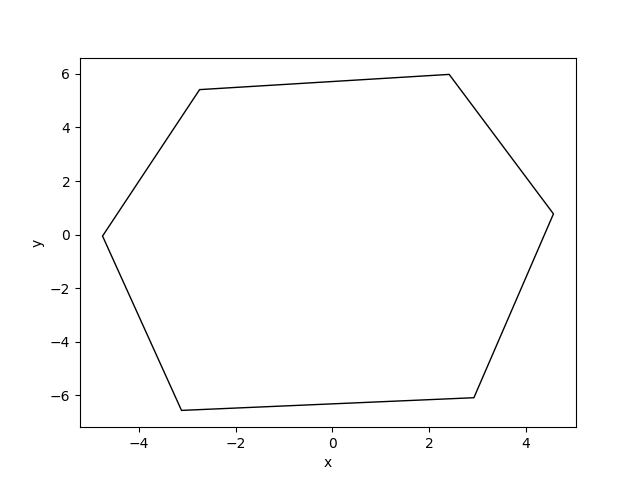
\includegraphics[scale=0.4]{res/pol_a.png}
        \caption{
            Wielokąt A
        }
    \end{subfigure}
    \begin{subfigure}[b]{0.46\textwidth}
        \centering
        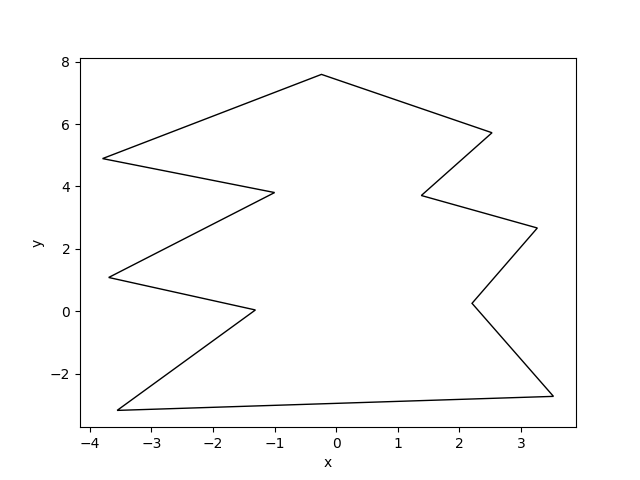
\includegraphics[scale=0.4]{res/pol_b.png}
        \caption{
            Wielokąt B
        }
    \end{subfigure}
    \begin{subfigure}[b]{0.46\textwidth}
        \centering
        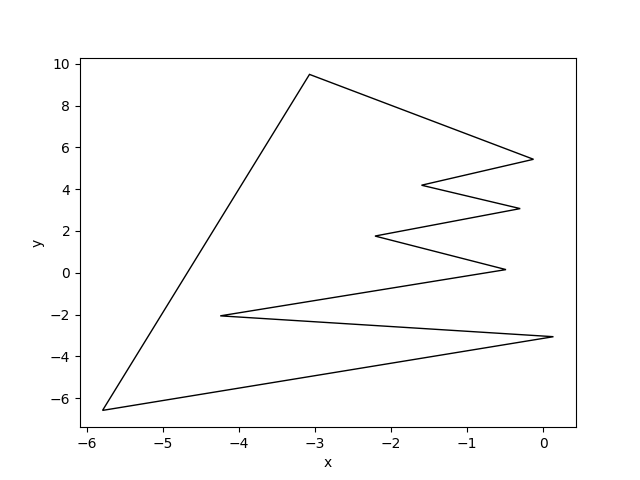
\includegraphics[scale=0.4]{res/pol_c.png}
        \caption{
            Wielokąt C
        }
    \end{subfigure}
    \begin{subfigure}[b]{0.46\textwidth}
        \centering
        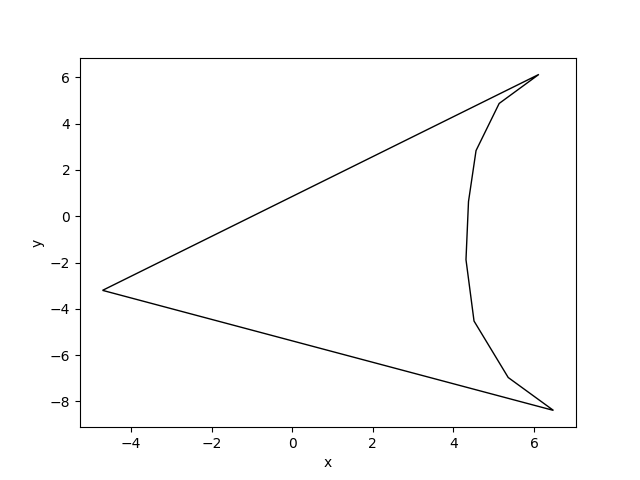
\includegraphics[scale=0.4]{res/pol_d.png}
        \caption{
            Wielokąt D
        }
    \end{subfigure}
    \begin{subfigure}[b]{0.46\textwidth}
        \centering
        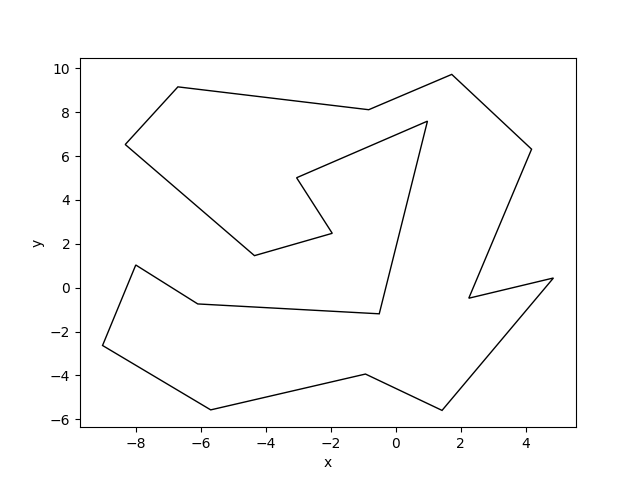
\includegraphics[scale=0.4]{res/pol_e.png}
        \caption{
            Wielokąt E
        }
    \end{subfigure}
    \caption{Wygenerowane zbiory}
\end{figure}

Ostatecznie przygotowałem aplikację umożliwiającą zadawanie dowolnych wielokątów
(w załączonym kodzie) oraz animacje wizualizujące działanie algorytmu triangulacji
(animacje są załączone razem ze sprawozdaniem).

\pagebreak

\section{Wyniki}
Przyjmuję następujące oznaczenia dla poszczególnych algorytmów:
\begin{itemize}
    \item \verb|is_y_monotonic| - sprawdzanie czy wielokąt jest y-monotoniczny.
    Wynikiem jest \verb|True| (prawda) lub \verb|False| (fałsz).
    \item \verb|color_vertex| - kategoryzacja wierzchołków. 
    Zwizualizowane wyniki dla poszczególnych wielokątów 
    zawarte są na Rysunkach: 2, 4, 6, 8, 10.
    Wierzchołki oznaczone są następującymi kolorami:
    \begin{enumerate}
        \item \textbf{Początkowe} - zielony
        \item \textbf{Końcowe} - czerwony
        \item \textbf{Łączące} - granatowy
        \item \textbf{Dzielące} - niebieski
        \item \textbf{Prawidłowe} - brązowy
    \end{enumerate}
    \item \verb|triangulate| - triangulacja wielokątów y-monotonicznych. 
    Zwizualizowane wyniki dla poszczególnych wielokątów zawarte są 
    na Rysunkach: 3, 5, 7, 9.
    (Wielokąt E nie jest monotoniczny, więc jest pominięty). W celu prostszej
    wizualizacji algorytm zwracał jedynie przekątne, które należy stworzyć
    (jako pary indeksów wierzchołków), implementacja zwracająca trójkąty
    (jako trójki indeksów wierzchołków) jest zawarta w załączonym kodzie.
    Stworzone przez algorytm przekątne oznaczone są kolorem czerwonym.
\end{itemize}

Załączone ze sprawozdaniem animacje przyjmują następujące oznaczenia:
\begin{itemize}
    \item Czerwone odcinki - przekątne stworzone przez algorytm.
    \item Czerwone punkty  - wierzchołki znajdujące się na stosie.
    \item Brązowe punkty - wierzchołki zdjęte ze stosu.
    \item Niebieskie punkty - wierzchołki jeszcze nie przetworzone przez algorytm. 
\end{itemize}

Sekcje od 3.1 do 3.5 zawierają wyniki algorytmów na poszczególnych
wielokątach, wraz z krótkim komentarzem na ich temat.

\pagebreak

\subsection{Wielokąt A}
Wielokąt ten pozwala nam sprawdzić czy algorytm poprawnie
radzi sobie z odfiltrowywaniem boków wielokąta z wyniku
(jest to konieczne jedynie kiedy zwracamy tylko 
stworzone przekątne). Ponadto pokazuje nam on czy algorytm
poprawnie radzi sobie gdy każdy kolejny rozważany
punkt należy do innego łańcucha.

Wyniki:

\verb|is_y_monotonic|: \verb|True|

\begin{minipage}{0.46\textwidth}
    \begin{figure}[H]
        \centering
        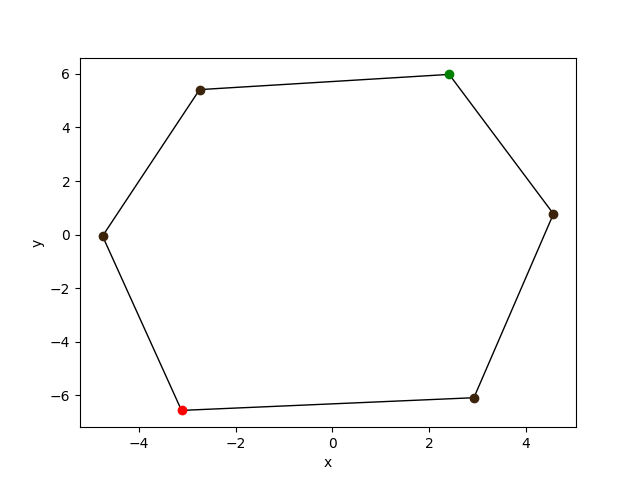
\includegraphics[scale=0.5]{res/pol_a_colors.png}
        \caption{Wynik \ttfamily color\_vertex \normalfont dla \\wielokąta A}
    \end{figure}
\end{minipage}
\begin{minipage}{0.46\textwidth}
    \begin{figure}[H]
        \centering
        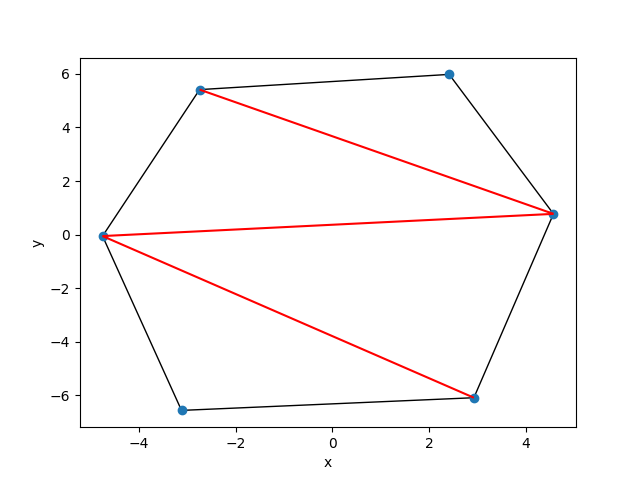
\includegraphics[scale=0.5]{res/pol_a_tri.png}
        \caption{Wynik \ttfamily triangulation \normalfont dla \\wielokąta A}
    \end{figure}
\end{minipage}

\subsection{Wielokąt B}
Wielokąt ten pozwala nam sprawdzić czy algorytm triangulacji
poprawnie radzi sobie w przypadku, gdy kolejno rozważane wierzchołki 
należą do różnych łańcuchów.

Wyniki:

\verb|is_y_monotonic|: \verb|True|

\begin{minipage}{0.46\textwidth}
    \begin{figure}[H]
        \centering
        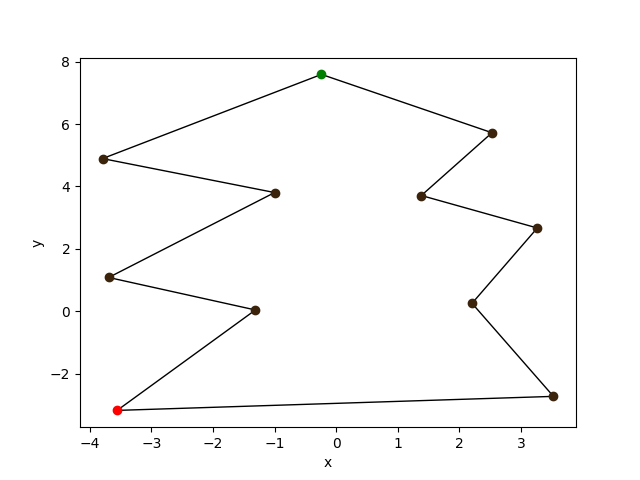
\includegraphics[scale=0.5]{res/pol_b_colors.png}
        \caption{Wynik \ttfamily color\_vertex \normalfont dla \\wielokąta B}
    \end{figure}
\end{minipage}
\begin{minipage}{0.46\textwidth}
    \begin{figure}[H]
        \centering
        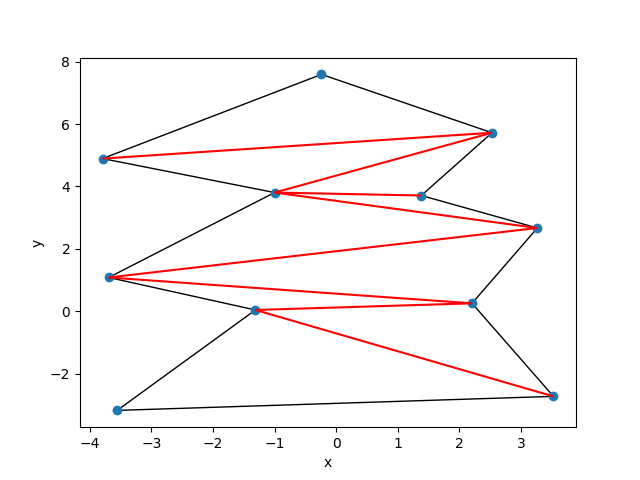
\includegraphics[scale=0.5]{res/pol_b_tri.png}
        \caption{Wynik \ttfamily triangulation \normalfont dla \\wielokąta B}
    \end{figure}
\end{minipage}

\subsection{Wielokąt C}
Wielokąt ten pozwala nam sprawdzić czy algorytm triangulacji
poprawnie radzi sobie w przypadku, gdy większość wierzchołków leży
na jednym łańcuchu, w którym tworzą trójkąty należące do wielokąta.

Wyniki:

\verb|is_y_monotonic|: \verb|True|

\begin{minipage}{0.46\textwidth}
    \begin{figure}[H]
        \centering
        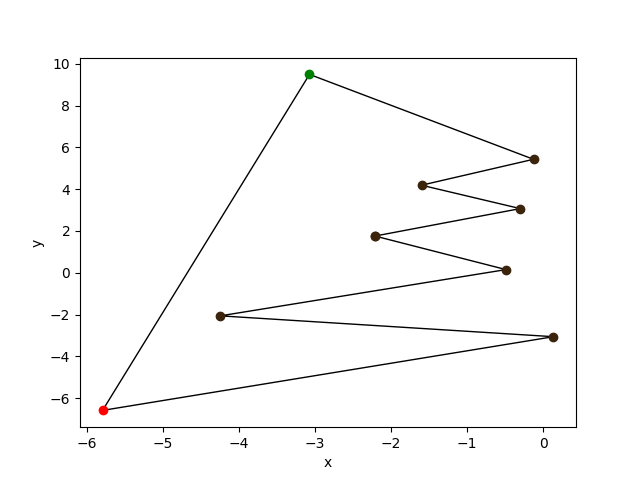
\includegraphics[scale=0.5]{res/pol_c_colors.png}
        \caption{Wynik \ttfamily color\_vertex \normalfont dla \\wielokąta C}
    \end{figure}
\end{minipage}
\begin{minipage}{0.46\textwidth}
    \begin{figure}[H]
        \centering
        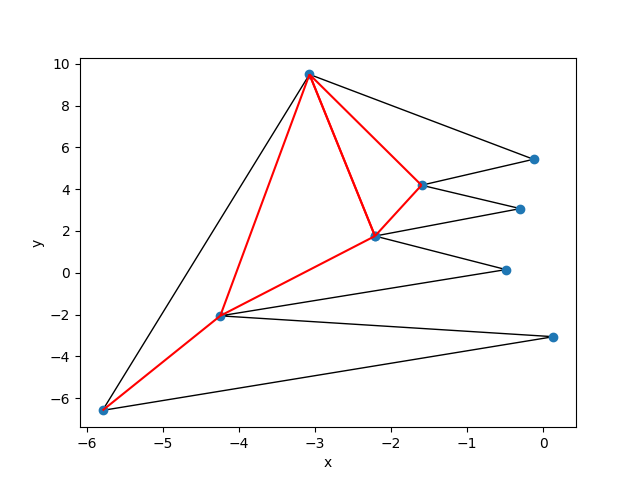
\includegraphics[scale=0.5]{res/pol_c_tri.png}
        \caption{Wynik \ttfamily triangulation \normalfont dla \\wielokąta C}
    \end{figure}
\end{minipage}

\subsection{Wielokąt D}
Wielokąt ten pozwala nam sprawdzić czy algorytm triangulacji
poprawnie radzi sobie w przypadku, gdy większość wierzchołków leży
na jednym łańcuchu, w którym tworzą trójkąty nie należące do wielokąta.

Wyniki:

\verb|is_y_monotonic|: \verb|True|

\begin{minipage}{0.46\textwidth}
    \begin{figure}[H]
        \centering
        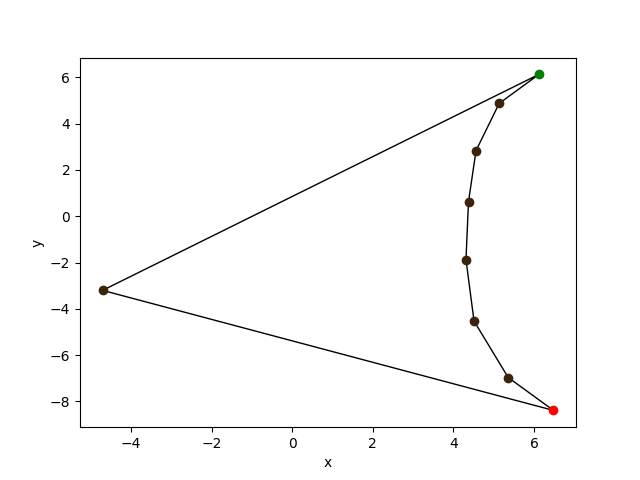
\includegraphics[scale=0.5]{res/pol_d_colors.png}
        \caption{Wynik \ttfamily color\_vertex \normalfont dla \\wielokąta D}
    \end{figure}
\end{minipage}
\begin{minipage}{0.46\textwidth}
    \begin{figure}[H]
        \centering
        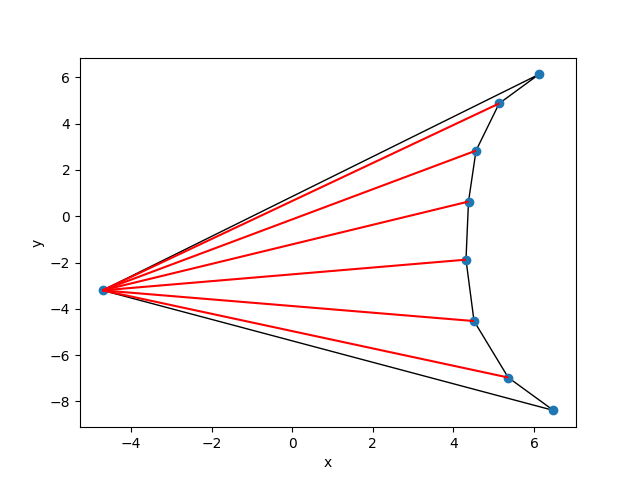
\includegraphics[scale=0.5]{res/pol_d_tri.png}
        \caption{Wynik \ttfamily triangulation \normalfont dla \\wielokąta D}
    \end{figure}
\end{minipage}

\subsection{Wielokąt E}
Wielokąt ten pozwala nam sprawdzić czy wielokąt niemonotoniczny
zostanie poprawnie sklasyfikowany i czy każdy typ wierzchołka jest
odpowiednio rozpoznawany.

Wyniki:

\verb|is_y_monotonic|: \verb|False|

\begin{figure}[H]
    \centering
    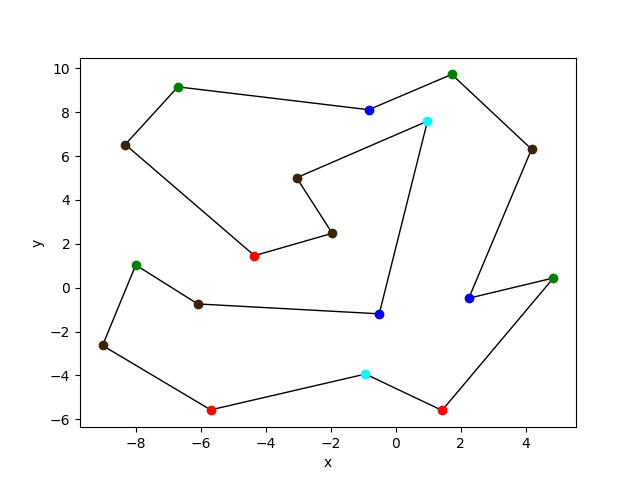
\includegraphics[scale=0.5]{res/pol_e_colors.png}
    \caption{Wynik \ttfamily color\_vertex \normalfont dla \\wielokąta E}
\end{figure}

\section{Podsumowanie}
Algorytmy zostały zaimplementowane prawidłowo, zarówno przechodząc wszystkie
testy jak i pokrywając się z przewidywaniami po wizualizacji. Wielokąty przedstawione
w sprawozdaniu zostały wybrane w celu wizualizacji działania algorytmu
i sprawdzenia jego poprawności w róznych przypadkach, opisanych 
w sprawozdaniu. Wygenerowane przez program wyniki zawarte są także
w załączonym kodzie, który generuje także listy znalezionych trójkątów 
dla każdego zbioru (reprezentowanych jako trójki indeksów wierzchołków).
Kod zawiera także funkcjonalność zadawania własnych wielokątów myszką
i sprawdzania na nich wyników wszystkich opisywanych algorytmów.
Wraz ze sprawozdaniem załączone są animacje przedstawiające poszczególne
kroki algorytmu triangulacji dla wielokątów A, B, C i D.

\end{document}
